\newpage
\setcounter{page}{1}
\pagenumbering{arabic}
\chapter{质点运动学}
\section{参考系}
\index{CKX@参考系}
描述质点运动时用的,固定在参考物上面的空间坐标系(如笛卡尔直角坐标系)和配置在各处的一套同步的钟构成一个参考系,通常就以选定的参考系命名,如太阳坐标系、地心坐标系、地面参考系等。

\section{运动函数}
\index{YDHS@运动函数}
\margin{其中$\bm{r}(t)$为质点在时刻$t$的径矢,即从坐标系原点指到时刻$t$质点所在位置的长度矢量。$x(t),y(t),z(t)$分别为径矢沿$x,y,z$轴的分量,也表示沿三个轴的分运动。左式表示运动的合成。}
相对于一定参数表示的质点位置随时间的变化的函数,即
\begin{equation}
\eq[\bm{r}=\bm{r}(t)=x(t) \,\bm{i} +y(t) \,\bm{j} +z(t)\, \bm{k}]
\end{equation}
\vspace{0.1cm}
\section{位移和速度}
\margin{\\[-1em] 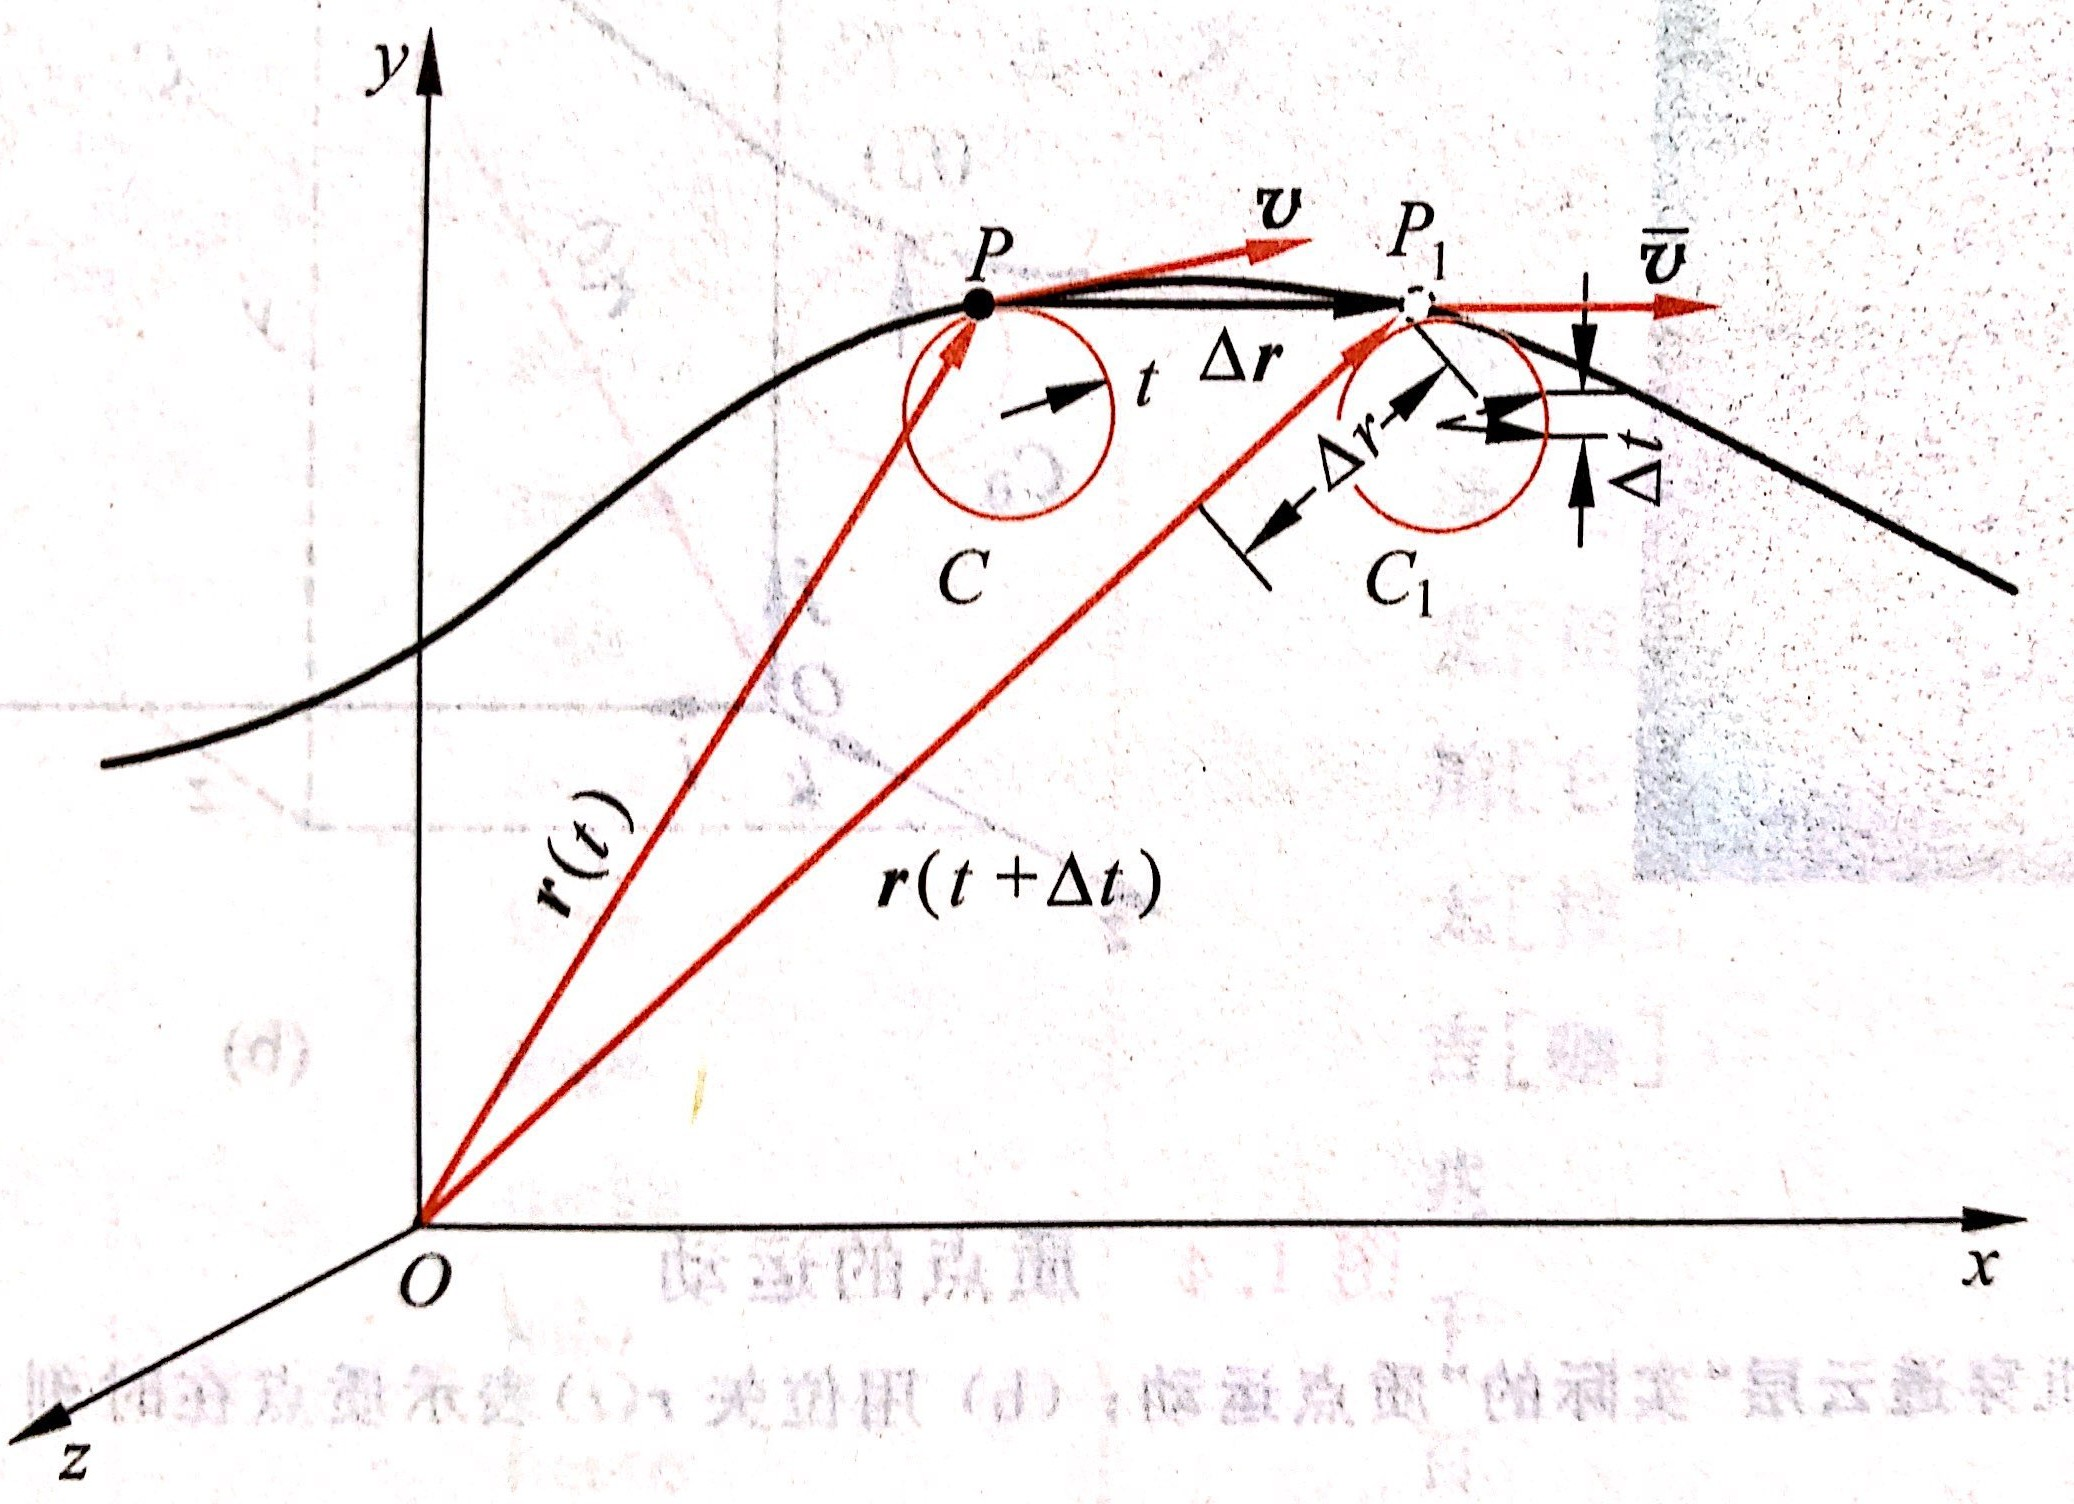
\includegraphics[width=1.1\linewidth]{picture/运1.jpg}\\$\d r = 0$说明作圆周运动\\$\d \bm{r}=0$说明作匀速运动}
\index{WY@位移}
\index{SD@速度}
质点在时间$\Delta t$内的位移为\eq[\Delta \bm{r}=\bm{r}(t+\Delta t)-\bm{r}(t).]\n
一般地
\begin{equation}
\eq
[
|\Delta \bm{r}| \neq \Delta r
]
\end{equation}

\n 质点在时刻$t$的速度为
\begin{equation}
\eq
[
\displaystyle \bm{v}=\frac{\d \bm{r} }{\d t}=\frac{\d x}{\d t} \,\bm{i} +\frac{\d y}{\d t} \,\bm{j} +\frac{\d z}{\d t}\, \bm{k}
]
\end{equation}
\margin{其中$\frac{\d x}{\d t} \,\bm{i} ,\frac{\d y}{\d t} \,\bm{j} ,\frac{\d z}{\rd t}\, \bm{k}$为代数量,其正负表示该分量与相应的坐标的方向相同或相反.速度方向沿质点运动轨迹的切线方向且指向运动的前方.}

\section{加速度和匀加速运动}
质点在时刻$t$的加速度\index{JSD@加速度}
\begin{equation}
\eq
[
\disp \bm{a}=\frac{\d \bm{v}}{\d t}=\frac{\d v_x}{\d t} \,\bm{i} +\frac{\d v_y}{\d t} \,\bm{j} +\frac{\d v_z}{\d t}\, \bm{k}
]
\end{equation}
\n 匀加速运动\index{YJSYD@匀加速运动}:
\margin{\quad \\ \hspace*{1.5em} 式中$(\bm{r_0},\bm{v_0})$是初值.}
\begin{equation}
\eq
[
\begin{cases}
\bm{v}=\bm{v_0}+\bm{a}t\\
\bm{r}=\bm{r_0}+\bm{v_0}t+\frac{1}{2}at^2
\end{cases}
\label{匀加速运动}
]
\end{equation}

\n 匀加速直线运动\index{YJSYD@匀加速直线运动}:即在式\eqref{匀加速运动}中取运动轨道为$x$轴,初始条件为$(x_0,v_0)$,则 
\begin{equation}
\eq[
\begin{cases}
v = v_0 +at\\
x=x_0+v_0t+\frac{1}{2}at^2\\
v^2-v_0^2=2ax
\end{cases}
]
\end{equation}

\section{抛体运动}
\dy[抛体运动]{PTYD}\jg
\par 抛体运动为平面运动,设运动平面为$xOy$平面,
\margin{抛体运动可以看成是沿竖直方向的匀加速运动和水平方向的匀速运动的合成}
$y$轴竖直向上,则有$a_x=0,a_y=-g$,以抛出点为原点,则
\begin{equation}
\begin{split}
&v_x=v_0\cos \theta ,\quad \quad v_y=v_0\sin\theta -gt\\
&x=v_0\cos \theta \cdot t,\quad \,\,\,y=v_0\sin \theta \cdot t-\frac{1}{2}gt^2
\end{split}
\end{equation}

\section{圆周运动}
\dy[圆周运动]{YZYD} \jg\jg
\par \quad \dy[线速度]{XSD}
\begin{equation}
\eq[v=\frac{\d s}{\d t}]
\end{equation}

\par \quad \dy[角速度]{JSD}
\begin{equation}
\eq[\omega =\frac{\d \theta }{\d t}=\frac{v}{R}]
\end{equation}

\par \quad \dy[角加速度]{JJSD}
\begin{equation}
\eq[\alpha =\frac{\d \omega }{\d t}]
\end{equation}

\par \quad \dy[加速度]{JSD}
\begin{equation}
\eq[\bm{a} =\bm{a}_n+\bm{a}_t]
\end{equation}

\par \quad \dy[法向加速度]{FXJSD}
\begin{equation}
\eq[a_n=\frac{v^2}{R}=R\omega^2]\quad \mbox{指向圆心}
\end{equation}

\par \quad \dy[切向加速度]{QXJSD}
\begin{equation}
\eq[a_t=\frac{\d v}{\d t}=R\alpha]\quad \mbox{沿切线方向}
\end{equation}

\newpage
\section{相对运动}
\dy[伽利略变换]{JLLBH}\jg
\margin{伽利略变换仅适用于$\bm{u}$远小于光速的情况.}
\par 运动的描述随所用的参考系的不同而不同,对于相对速度为$\bm{u}$的两个参考系$(S,S')$,同一质点$A$\jg
\margin{在这三个位移下标中,前一个字母表示运动的物体,后一字母表示参考系.}
\par \quad \dy[位移变换]{WYBH}
\begin{equation}
\Delta \bm{r}_{AE}=\Delta \bm{r}_{AS}+\Delta \bm{r}_{SE}
\end{equation}

\par \quad \dy[速度变换]{WYBH}
\margin{$v_a$为绝对速度\\\kg$v_r$为相对速度\\\kg$u$为牵连速度}
\begin{equation}
\bm{v_a}=\bm{v_r}+\bm{u}
\end{equation}

\par \quad \dy[加速度变换]{WYBH}
\begin{equation}
\bm{a} = \bm{a}'+\bm{a}_0,\quad \bm{a}_0=\frac{\d \bm{u}}{\d t}
\end{equation}
\par 特别地,当$a_0 = 0$时,
\begin{equation*}
\bm{a}=\bm{a'}
\end{equation*}



